% Options for packages loaded elsewhere
\PassOptionsToPackage{unicode}{hyperref}
\PassOptionsToPackage{hyphens}{url}
%
\documentclass[
  ignorenonframetext,
]{beamer}
\usepackage{pgfpages}
\setbeamertemplate{caption}[numbered]
\setbeamertemplate{caption label separator}{: }
\setbeamercolor{caption name}{fg=normal text.fg}
\beamertemplatenavigationsymbolshorizontal
% Prevent slide breaks in the middle of a paragraph
\widowpenalties 1 10000
\raggedbottom
\setbeamertemplate{part page}{
  \centering
  \begin{beamercolorbox}[sep=16pt,center]{part title}
    \usebeamerfont{part title}\insertpart\par
  \end{beamercolorbox}
}
\setbeamertemplate{section page}{
  \centering
  \begin{beamercolorbox}[sep=12pt,center]{part title}
    \usebeamerfont{section title}\insertsection\par
  \end{beamercolorbox}
}
\setbeamertemplate{subsection page}{
  \centering
  \begin{beamercolorbox}[sep=8pt,center]{part title}
    \usebeamerfont{subsection title}\insertsubsection\par
  \end{beamercolorbox}
}
\AtBeginPart{
  \frame{\partpage}
}
\AtBeginSection{
  \ifbibliography
  \else
    \frame{\sectionpage}
  \fi
}
\AtBeginSubsection{
  \frame{\subsectionpage}
}

\usepackage{amsmath,amssymb}
\usepackage{iftex}
\ifPDFTeX
  \usepackage[T1]{fontenc}
  \usepackage[utf8]{inputenc}
  \usepackage{textcomp} % provide euro and other symbols
\else % if luatex or xetex
  \usepackage{unicode-math}
  \defaultfontfeatures{Scale=MatchLowercase}
  \defaultfontfeatures[\rmfamily]{Ligatures=TeX,Scale=1}
\fi
\usepackage{lmodern}
\usetheme[]{default}
\ifPDFTeX\else  
    % xetex/luatex font selection
\fi
% Use upquote if available, for straight quotes in verbatim environments
\IfFileExists{upquote.sty}{\usepackage{upquote}}{}
\IfFileExists{microtype.sty}{% use microtype if available
  \usepackage[]{microtype}
  \UseMicrotypeSet[protrusion]{basicmath} % disable protrusion for tt fonts
}{}
\makeatletter
\@ifundefined{KOMAClassName}{% if non-KOMA class
  \IfFileExists{parskip.sty}{%
    \usepackage{parskip}
  }{% else
    \setlength{\parindent}{0pt}
    \setlength{\parskip}{6pt plus 2pt minus 1pt}}
}{% if KOMA class
  \KOMAoptions{parskip=half}}
\makeatother
\usepackage{xcolor}
\newif\ifbibliography
\setlength{\emergencystretch}{3em} % prevent overfull lines
\setcounter{secnumdepth}{-\maxdimen} % remove section numbering


\providecommand{\tightlist}{%
  \setlength{\itemsep}{0pt}\setlength{\parskip}{0pt}}\usepackage{longtable,booktabs,array}
\usepackage{calc} % for calculating minipage widths
\usepackage{caption}
% Make caption package work with longtable
\makeatletter
\def\fnum@table{\tablename~\thetable}
\makeatother
\usepackage{graphicx}
\makeatletter
\def\maxwidth{\ifdim\Gin@nat@width>\linewidth\linewidth\else\Gin@nat@width\fi}
\def\maxheight{\ifdim\Gin@nat@height>\textheight\textheight\else\Gin@nat@height\fi}
\makeatother
% Scale images if necessary, so that they will not overflow the page
% margins by default, and it is still possible to overwrite the defaults
% using explicit options in \includegraphics[width, height, ...]{}
\setkeys{Gin}{width=\maxwidth,height=\maxheight,keepaspectratio}
% Set default figure placement to htbp
\makeatletter
\def\fps@figure{htbp}
\makeatother

\usepackage{fontspec}
\usepackage{graphicx}
\usepackage{grffile}
\makeatletter
\@ifpackageloaded{caption}{}{\usepackage{caption}}
\AtBeginDocument{%
\ifdefined\contentsname
  \renewcommand*\contentsname{Table of contents}
\else
  \newcommand\contentsname{Table of contents}
\fi
\ifdefined\listfigurename
  \renewcommand*\listfigurename{List of Figures}
\else
  \newcommand\listfigurename{List of Figures}
\fi
\ifdefined\listtablename
  \renewcommand*\listtablename{List of Tables}
\else
  \newcommand\listtablename{List of Tables}
\fi
\ifdefined\figurename
  \renewcommand*\figurename{Figure}
\else
  \newcommand\figurename{Figure}
\fi
\ifdefined\tablename
  \renewcommand*\tablename{Table}
\else
  \newcommand\tablename{Table}
\fi
}
\@ifpackageloaded{float}{}{\usepackage{float}}
\floatstyle{ruled}
\@ifundefined{c@chapter}{\newfloat{codelisting}{h}{lop}}{\newfloat{codelisting}{h}{lop}[chapter]}
\floatname{codelisting}{Listing}
\newcommand*\listoflistings{\listof{codelisting}{List of Listings}}
\makeatother
\makeatletter
\makeatother
\makeatletter
\@ifpackageloaded{caption}{}{\usepackage{caption}}
\@ifpackageloaded{subcaption}{}{\usepackage{subcaption}}
\makeatother

\ifLuaTeX
  \usepackage{selnolig}  % disable illegal ligatures
\fi
\usepackage{bookmark}

\IfFileExists{xurl.sty}{\usepackage{xurl}}{} % add URL line breaks if available
\urlstyle{same} % disable monospaced font for URLs
\hypersetup{
  pdftitle={Class 30},
  pdfauthor={Sarah E. Grabinski},
  hidelinks,
  pdfcreator={LaTeX via pandoc}}


\title{Class 30}
\subtitle{DATA1220-55, Fall 2024}
\author{Sarah E. Grabinski}
\date{2024-11-18}

\begin{document}
\frame{\titlepage}


\begin{frame}{Analysis Tools (So Far)}
\phantomsection\label{analysis-tools-so-far}
\begin{itemize}
\tightlist
\item
  1-sample proportion- or \(Z\)-test for a single proportion
\end{itemize}

\pause

\begin{itemize}
\tightlist
\item
  2-sample proportion- or \(Z\)-test for the difference between 2
  proportions
\end{itemize}

\pause

\begin{itemize}
\tightlist
\item
  Chi-squared test for independence between 2 categorical variables
\end{itemize}

\pause

\begin{itemize}
\tightlist
\item
  1 sample \(t\)-test for a single mean
\end{itemize}

\pause

\begin{itemize}
\tightlist
\item
  Paired means \(t\)-test for the difference between 2 means from same
  unit
\end{itemize}

\pause

\begin{itemize}
\tightlist
\item
  2-sample \(t\)-test for the difference between 2 unpaired means
\end{itemize}
\end{frame}

\begin{frame}{Remaining Tools}
\phantomsection\label{remaining-tools}
\begin{itemize}
\tightlist
\item
  ANOVA test for the difference between 3+ unpaired means
\end{itemize}

\pause

\begin{itemize}
\tightlist
\item
  Pearson correlation test for dependence between 2 numeric variables
\end{itemize}

\pause

\begin{itemize}
\tightlist
\item
  Linear regression for dependence between 1 or more explanatory
  variables (numeric or categorical) and a numerical or binary (0/1)
  response variable (if time)
\end{itemize}

\pause

\begin{itemize}
\tightlist
\item
  Developing a research question with a testable hypothesis
\end{itemize}

\pause

\begin{itemize}
\tightlist
\item
  Communicating statistical methods and analysis results
\end{itemize}

\pause

\begin{itemize}
\tightlist
\item
  Data visualization tips \& tricks, do's \& dont's
\end{itemize}

\pause

\begin{itemize}
\tightlist
\item
  Statistical analysis best practice
\end{itemize}
\end{frame}

\begin{frame}{ANOVA and the F-Test for Comparing 3+ Means}
\phantomsection\label{anova-and-the-f-test-for-comparing-3-means}
\begin{itemize}
\tightlist
\item
  The ANOVA test (\textbf{\emph{An}}alysis \textbf{\emph{o}}f
  \textbf{\emph{Va}}riance) tests for a difference between the means
  \(\mu_i\) of \(k\) groups (\(k \ge 3\)).
\end{itemize}

\pause

\begin{itemize}
\item
  Compares the ratio of the \textbf{\emph{between-group}} variability in
  means to what would be expected based on the
  \textbf{\emph{within-group}} variability in the means.

  \[
    \text{test statistic}=\frac{\text{Between-Groups Variability/Error}}{\text{Within-Groups Variability/Error}}
  \]
\end{itemize}

\pause

\begin{itemize}
\tightlist
\item
  The probability of the observed difference in between-group
  variability vs within-group variability is calculated using the \(F\)
  distribution.
\end{itemize}

\pause

\begin{itemize}
\tightlist
\item
  Rarely calculated by hand. We will perform these exclusively with R.
\end{itemize}
\end{frame}

\begin{frame}{ANOVA F-Test Hypotheses}
\phantomsection\label{anova-f-test-hypotheses}
\begin{itemize}
\item
  Null hypothesis: the mean outcome \(\mu_i\) is the same across all
  \(k\) groups, such that each group has the same population mean
  \(\mu\).

  \[
    H_0 \colon \mu_1=\mu_2=...=\mu_k=\mu
  \]
\end{itemize}

\pause

\begin{itemize}
\item
  Alternate hypothesis: at least one mean \(\mu_i\) is different from
  the other \(k-1\) means, such that there is no single population mean
  \(\mu\).

  \[
    H_A \colon \text{At least 1 } \mu_i \ne \mu
  \]
\end{itemize}
\end{frame}

\begin{frame}{Assumptions}
\phantomsection\label{assumptions}
\begin{enumerate}
\tightlist
\item
  \textbf{\emph{Independent \& Identically Distributed Observations}}:
  Observations are independent both within and between groups and
  identically distributed within groups.
\end{enumerate}

\pause

\begin{enumerate}
\setcounter{enumi}{1}
\tightlist
\item
  \textbf{\emph{Sample size}}: There are more than 30 observations in
  each of the \(k\) groups (\(n_i \ge 30\)).
\end{enumerate}

\pause

\begin{enumerate}
\setcounter{enumi}{2}
\tightlist
\item
  \textbf{\emph{Normality}}: Especially when \(n_i\) are small, data
  within each of the \(k\) groups is normally distributed. This
  condition relaxes as \(n_i\) increases (\(n_i \to \infty\)).
\end{enumerate}

\pause

\begin{enumerate}
\setcounter{enumi}{3}
\tightlist
\item
  \textbf{\emph{Equal variance}}: Within-group variance is approximately
  equal across the \(k\) groups. This condition relaxes as sample sizes
  \(n_i\) become more balanced between the \(k\) groups
  (\(\frac{n}{k} \to n_i\)).
\end{enumerate}
\end{frame}

\begin{frame}{The F-Distribution}
\phantomsection\label{the-f-distribution}
\begin{itemize}
\item
  2 degree of freedom parameters

  \begin{itemize}
  \item
    The number of groups \(k\) minus 1: \(\text{df}_1=k-1\)
  \item
    The number of observations \(n\) minus the number of groups \(k\):
    \(\text{df}_2=n-k\)
  \end{itemize}
\end{itemize}

\pause

\begin{itemize}
\tightlist
\item
  The larger the test statistic \(F\), the less likely the observed data
  is under the null hypothesis
\end{itemize}

\pause

\begin{itemize}
\tightlist
\item
  Like the Chi-squared (\(\chi^2\)) distribution, the upper tail
  probability is always used for hypothesis testing
\end{itemize}
\end{frame}

\begin{frame}{The F-Distribution}
\phantomsection\label{the-f-distribution-1}
\begin{columns}[T]
\begin{column}{0.5\textwidth}
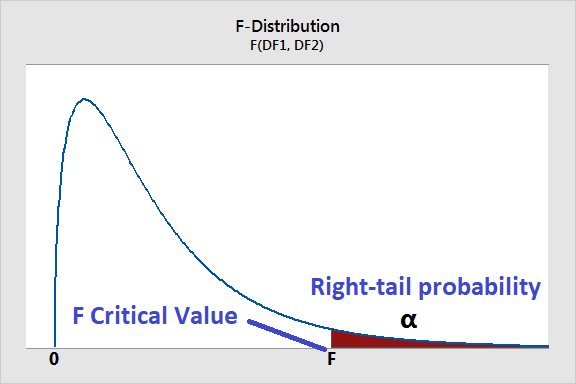
\includegraphics{class30_files/mediabag/f-distribution.png}
\end{column}

\begin{column}{0.5\textwidth}
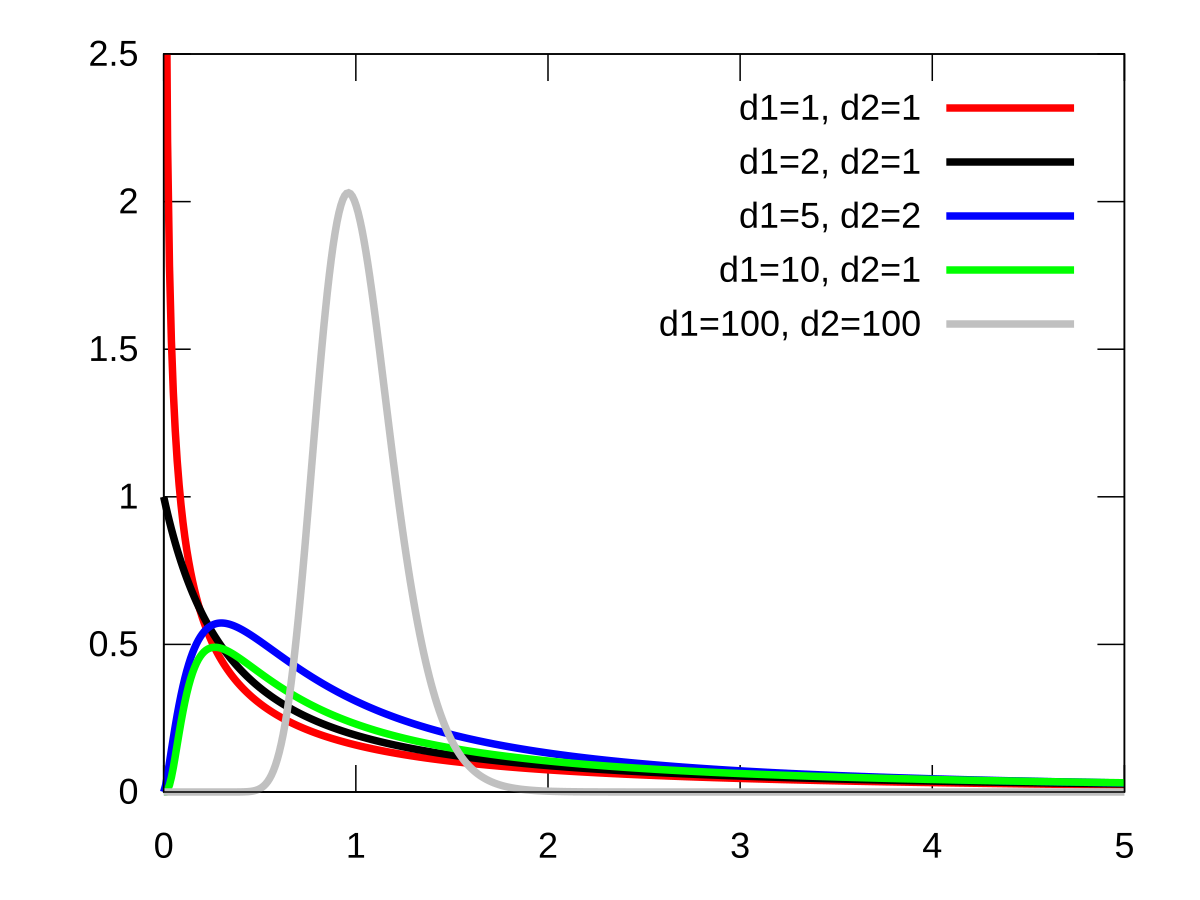
\includegraphics{class30_files/mediabag/f-distribution2.png}
\end{column}
\end{columns}
\end{frame}

\begin{frame}{ANOVA Results Table}
\phantomsection\label{anova-results-table}
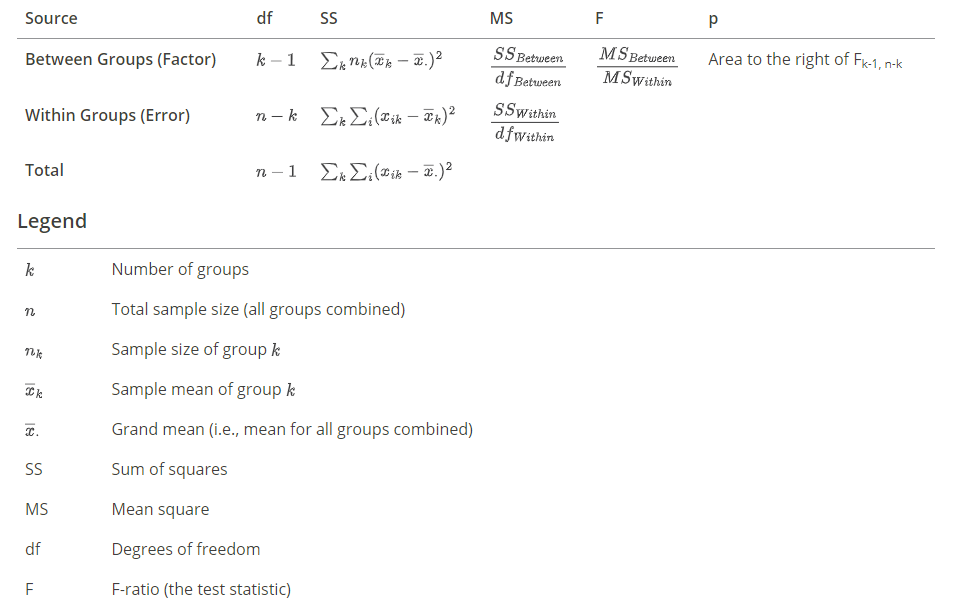
\includegraphics{class30_files/mediabag/anova-calculation-ta.png}
\end{frame}

\begin{frame}{Example: Wolf River Sediments}
\phantomsection\label{example-wolf-river-sediments}
\begin{columns}[T]
\begin{column}{0.48\textwidth}
\begin{itemize}
\tightlist
\item
  The Wolf River in Tennessee flows past an abandoned site once used by
  the pesticide industry for dumping wastes, including chlordane
  (pesticide), aldrin, and dieldrin (both insecticides)
\item
  These highly toxic organic compounds can cause various cancers and
  birth defects
\item
  The standard methods to test whether these substances are present in a
  river is to take samples at six-tenths depth
\item
  Since these compounds are denser than water and their molecules tend
  to stick to particles of sediment, they are more likely to be found in
  higher concentrations near the bottom
\end{itemize}
\end{column}

\begin{column}{0.48\textwidth}
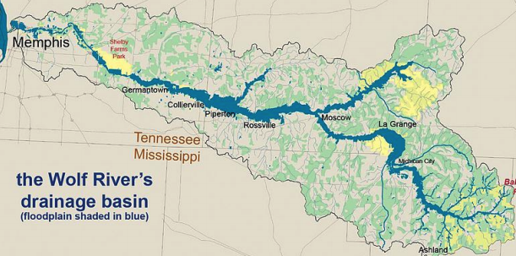
\includegraphics{class30_files/mediabag/wolf-river-map.png}
\end{column}

\textbf{\emph{Research Question:}} Does the average aldrin concentration
vary between the bottom, mid-depth, and surface?

\begin{frame}{The Data}
\phantomsection\label{the-data}
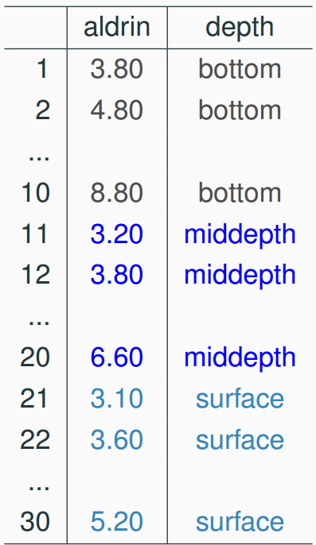
\includegraphics{class30_files/mediabag/concentration-table.png}
\end{frame}

\begin{frame}{Exploratory Analysis \& Sample Statistics}
\phantomsection\label{exploratory-analysis-sample-statistics}
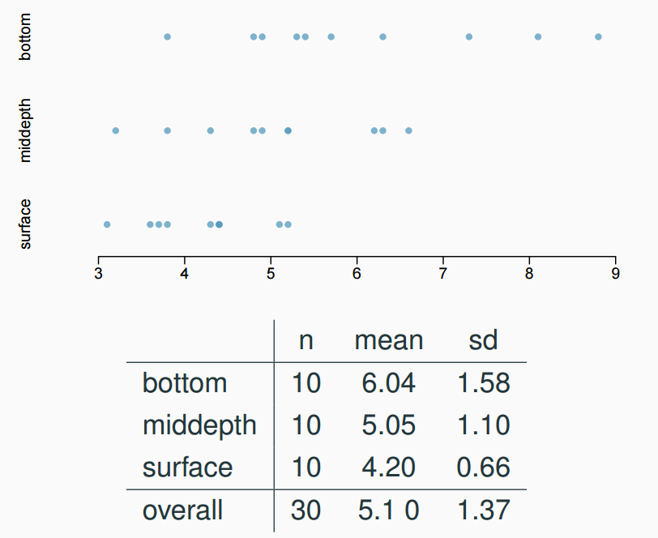
\includegraphics{class30_files/mediabag/summary-statistics.png}
\end{frame}

\begin{frame}{Equal Variance Assumption}
\phantomsection\label{equal-variance-assumption}
\begin{figure}[H]

{\centering 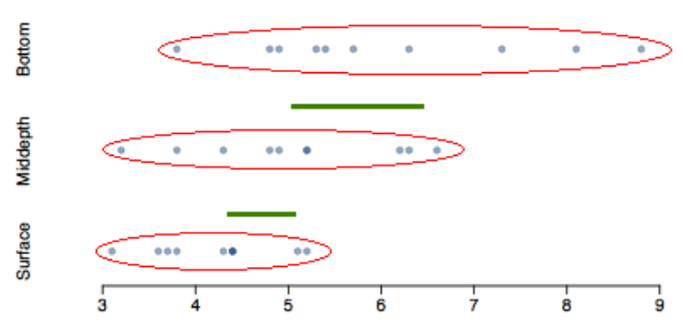
\includegraphics{class30_files/mediabag/variance.png}

}

\caption{Do these variances look approximately equal?}

\end{figure}%
\end{frame}

\begin{frame}{ANOVA Results}
\phantomsection\label{anova-results}
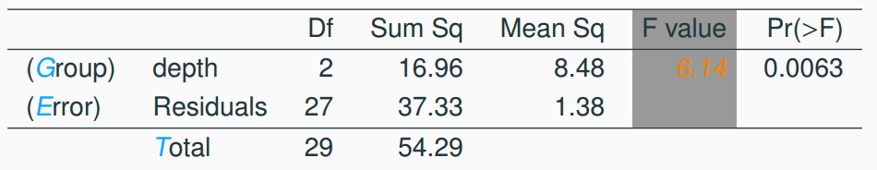
\includegraphics{class30_files/mediabag/example-anova-output.png}
\end{frame}

\begin{frame}{Interpreting The Results}
\phantomsection\label{interpreting-the-results}
\begin{itemize}
\tightlist
\item
  The test statistic \(F\) was 6.14, meaning the between-groups
  variability was 6.14 times as large as the within-group variability.
\end{itemize}

\pause

\begin{itemize}
\tightlist
\item
  The p-value was 0.0063, meaning it was very unlikely to have seen this
  much variability between groups in samples of these sizes, given the
  null hypothesis that each mean is the same (\(\mu_i=\mu\)).
\end{itemize}

\pause

\begin{itemize}
\tightlist
\item
  The p-value is less than a significance threshold of \(\alpha=0.05\),
  so we would reject the null hypothesis that the means of the 3 groups
  are equal. The mean of at least one group differs from the other
  means.
\end{itemize}

\pause

\begin{itemize}
\tightlist
\item
  But we made some pretty strong assumptions.
\end{itemize}

\pause

\begin{itemize}
\tightlist
\item
  If you want to know which means are different from each other, you
  will have to do additional pairwise tests between group means.
\end{itemize}
\end{frame}
\end{columns}
\end{frame}




\end{document}
